\documentclass[../main/report.tex]{subfiles}
\begin{document}

\chapter{Results}

\begin{figure}[H]
	\centering
	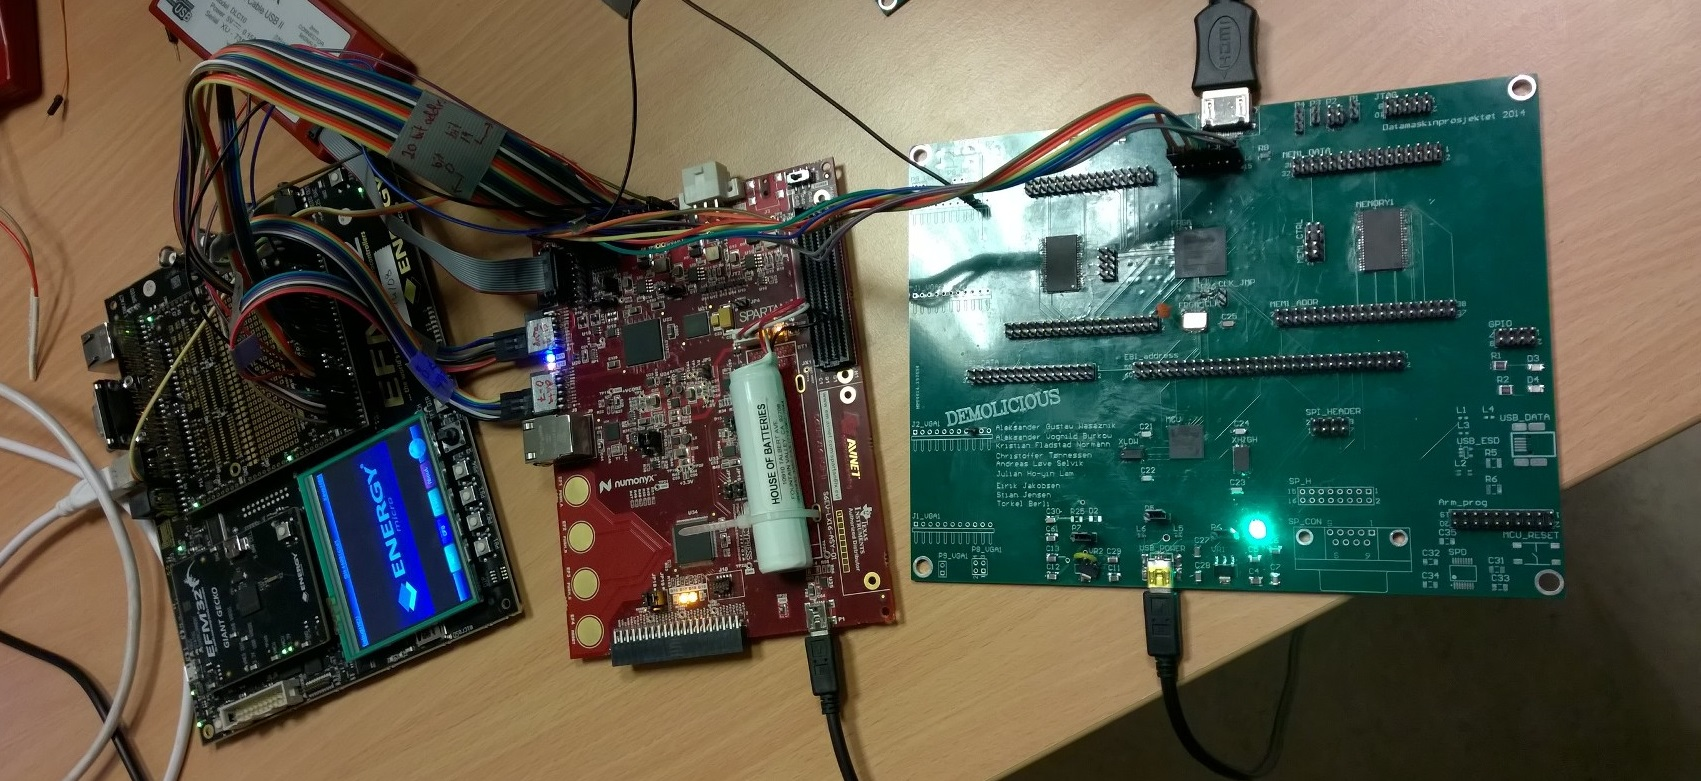
\includegraphics[width=\textwidth]{../results/diagrams/frankenlicious.jpeg}
	\caption{The working Demolicious devkit setup}
	\label{fig:frankenlicious}
\end{figure}

In this section, the fruit of our labor, namely the Demolicious system is presented.
The system has been sucessfully run on a concoction of FPGA and MCU devkits, using the HDMI port of the PCB for video output.
This setup is showcased in figure \ref{fig:frankenlicious}.

A PCB version is almost fully operational.
A version with both FPGA and MCU flashed with their respective images managed to output animations, with some undiagnosed showstopping software glitches.
The venture had to be paused due to a lack of time towards the end of the project.

Kernel images presented in this section are taken from the same setup presented in figure \ref{fig:frankenlicious}.

\section{Scalability of the Demolicious system}
\label{sec:scalability}

The architecture of the Demolicious system easily scales to a larger number of processors.
As there is a linear relationship between the number of processor cores on chip and processor throughput, one can simply add more cores to increase performance.

Limiting factors to this scalability include:
\begin{enumerate}
  \item
    The more cores, the lower the clock frequency, as signal propagation time and fanout increases
  \item
    Space available on the chosen FPGA
  \item
    Power consumption constraints, as more cores increase active power consumption
\end{enumerate}

\begin{table}[H]
\begin{tabularx}{\textwidth}{cccccc}
\hline
Cores & Crit. path & Max freq. & Dynamic+quiescent power & LX16 & LX45 \\
\hline
\hline
2      & 17.103ns      & 58.469MHz & \SI{0.272}{W}: 0.088 + 0.184 & \checkmark & \checkmark  \\
4     & 17.959ns      & 55.682MHz & \SI{0.292}{W}: 0.107 + 0.184 & \checkmark & \checkmark \\
8   & 19.722ns      & 50.108MHz & \SI{0.353}{W}: 0.168 + 0.186 & X          & \checkmark \\
16     & X  & X & X        & X & X \\
       &               &           &                   &    & \\
\hline
\end{tabularx}
\caption{Hardware configurations compared. Harvested from post place \& route static simulation.}
\label{table:scalability}
\end{table}

The 4-core design fits with room to spare on the LX16, but the 8-core design does not fit.
The LX45 shifts this up one notch, fitting the 8-core design, but being unable to place \& route the 16-core design.
For all processor designs, the critical path passes from the immediate field of the instruction through the ALU into the active register file.
This is something that could be decreased drastically by pipelining the processor.

Figure \ref{table:scalability} shows that there is a negligible drop in maximum frequency from two to eight cores.
At 50.108MHz with 8 cores, the GPU has an instruction throughput of ~400 MIPS.
This compares favorably to the ~117 MIPS of the two-core architecture.

It does however come with a 100mAh increase in power draw.
Luckily this only constitutes a 30\% total increase in power, considerably less than the fourfold improvement in GPU throughput.

\section{Performance}

In the Demolicious system, kernel calls can be issued by the CPU, taking only a few cycles.
This means that the number of frames per second (FPS) that the system can display is dominated by the run time of the kernels.

\begin{figure}[H]
	\centering
	\begin{subfigure}[t]{0.45\textwidth}
		\centering
		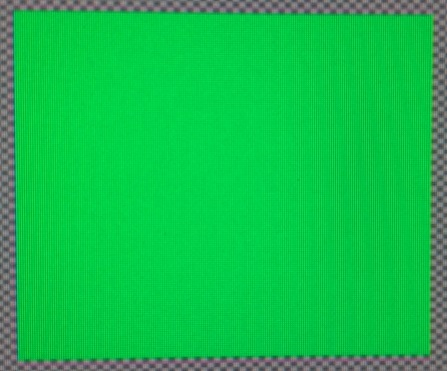
\includegraphics[width=\textwidth]{../results/diagrams/green_screen_run.jpg}
		\caption{Output from the green screen kernel.}
	\end{subfigure} 
	\begin{subfigure}[t]{0.45\textwidth}
		\centering
		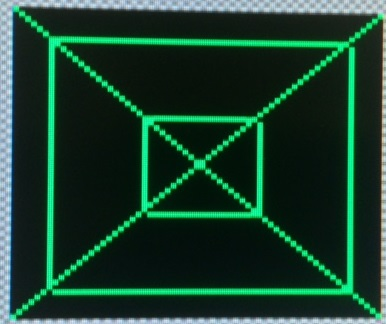
\includegraphics[width=\textwidth]{../results/diagrams/kernel_run_tunnel.jpg}
		\caption{Output from the tunnel kernel.}
	\end{subfigure}
	\caption{Running two example kernels.}
	\label{fig:kernel_outputs}
\end{figure}

Figure \ref{fig:kernel_outputs} shows the output from the green screen kernel, and a more complex tunnel effect kernel (listing \ref{lst:tunnel-kernel}).
It's desirable that both these kernels can be run at about 30 FPS.
Using the results presented in section \ref{sec:scalability}, the expected frames per second for varying resolutions can be estimated.

\begin{figure}[H]
	\centering
		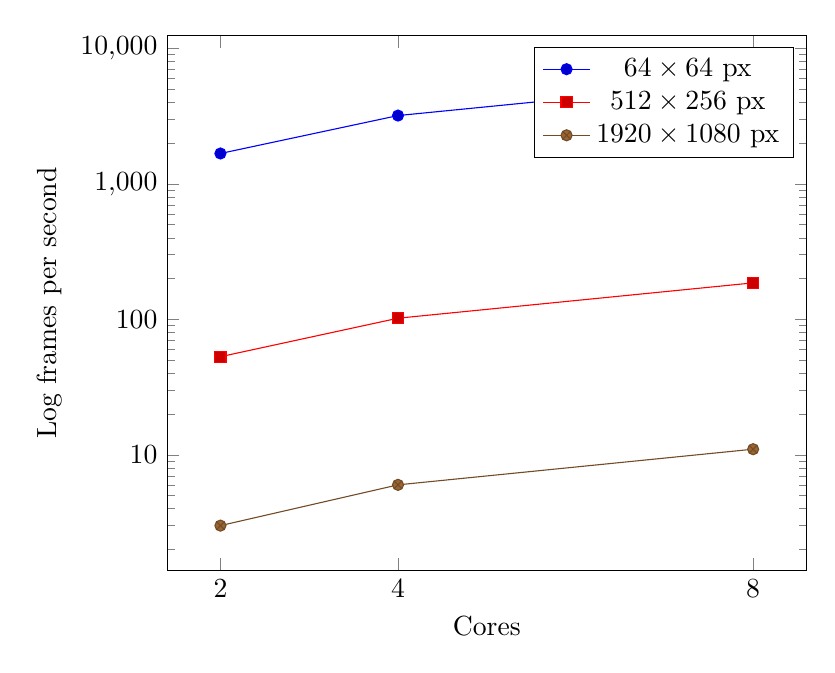
\begin{tikzpicture}
		   \begin{semilogyaxis}[
		   	   width=0.8\textwidth,
			   log ticks with fixed point,
		       xlabel=Cores,
		       ylabel=Log frames per second,
		       xtick = {2,4,8}
		   ]

		     \addplot plot coordinates {
		      	(2, 1678)
		      	(4, 3198)
    			(8, 5813)

             };

		   \addplot plot coordinates {
		      (2, 53)
		      (4, 102)
		      (8, 186)
		   };

		   \addplot plot coordinates {
		      (2, 3)
		      (4, 6)
		      (8, 11)
		   };

		   \legend{
		   $64\times64$ px \\
		   $512\times256$ px\\
		   $1920\times1080$ px\\}

		   \end{semilogyaxis}
		\end{tikzpicture}
		\caption{Running the green screen kernel.}
		\label{fig:kernel_green_screen_fps}
\end{figure}
\begin{figure}[H]
	\centering
	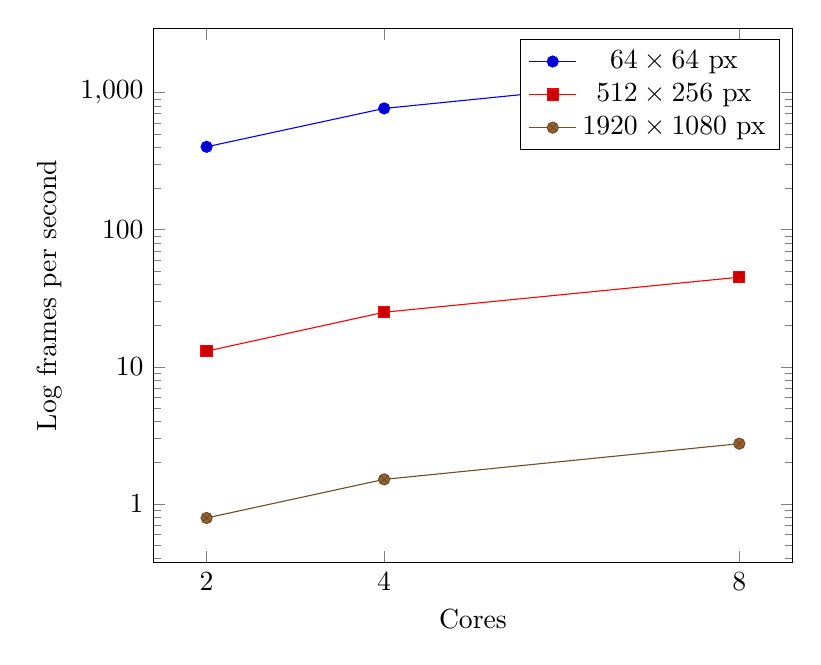
\begin{tikzpicture}
	 \begin{semilogyaxis}[
	 	 width=0.8\textwidth,
	     log ticks with fixed point,
	     xlabel=Cores,
	     ylabel=Log frames per second,
		     xtick = {2,4,8}
		 ]
		 \addplot plot coordinates {
		    (2, 402)
		    (4, 766)
		    (8, 1394)
		 };
		 \addplot plot coordinates {
		    (2, 13)
		    (4, 25 )
		    (8, 45)
		 };
		 \addplot plot coordinates {
		    (2, 0.79)
		    (4, 1.51)
		    (8, 2.75)
		 };
 
 
		 \legend{$64\times64$ px\\
		 $512\times256$ px\\
		 $1920\times1080$ px\\}

		 \end{semilogyaxis}
	\end{tikzpicture}
	\caption{Running the tunnel kernel.}
	\label{fig:kernel_tunnel_fps}
\end{figure}


The figures \ref{fig:kernel_tunnel_fps}, and \ref{fig:kernel_green_screen_fps} display the relationship between frame rate, resolution and number of cores.
Both figures display that doubling the amount of core roughly doubles the frame rate.

For a configuration of cores, the time it takes to process one pixel is constant.
This means that the time to execute one kernel scales linearly with the resolution.
When the output resolution is increased, the amount of pixels to process increases quadratically.
As a consequence the frame rate decreases quadratically when the resolution grows.
  
For the target resolution for the project, which is $512\times256$, the project goal of maintaining 30 fps is achieved.

\section{Video output}
The Demolicious system can output to a screen using HDMI.
The minimum resolution permitted by the HDMI protocol is $640\times480$,
but the size of the data memory limits the actual resolution to $512\times256$ pixels.
The rest of the screen is padded with a checker pattern.
Most of the time the output image is correct.
However, the output image is distorted under certain conditions.
\begin{figure}[H]
	\centering
	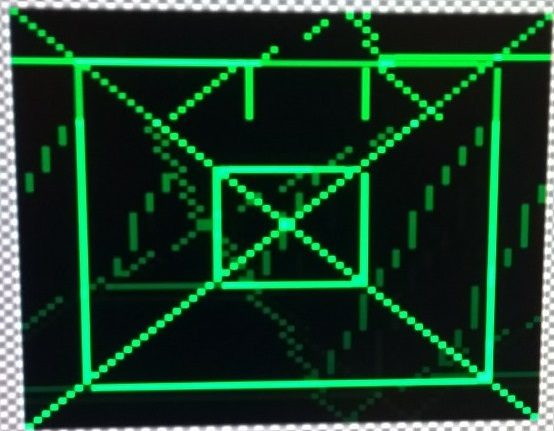
\includegraphics[width=0.8\textwidth]{../results/diagrams/flicker.jpg}
	\caption{Flickering when running the tunnel kernel. This picture was exposed over two frames.}
	\label{fig:flickering}
\end{figure}
Some kernels exhibit intermittent flickering (Figure \ref{fig:flickering}).
The exact reason for why this occurs is unclear, but
it can be observed that the flicker contains parts of the last frame. 
This may be caused by a failure in the synchronization mechanism in the video unit.

Since the GPU has priority on memory access, the video unit may get starved for data.
When the video unit is starved the buffer containing pixels to output will underflow.
For the duration of the starve, a line containing the previous pixel on the bus will be displayed on the screen.

\section{Single vs double buffering}

Screen tearing is a visual artifact where parts of two consecutive frames are displayed at the same time.
This occurs because the video unit reads the frame buffer before the GPU has finished rendering it.  
In figure \ref{fig:single_buffering} the artifact can be observed, occurrences are marked with red circles.

\begin{figure}[H]
	\centering
	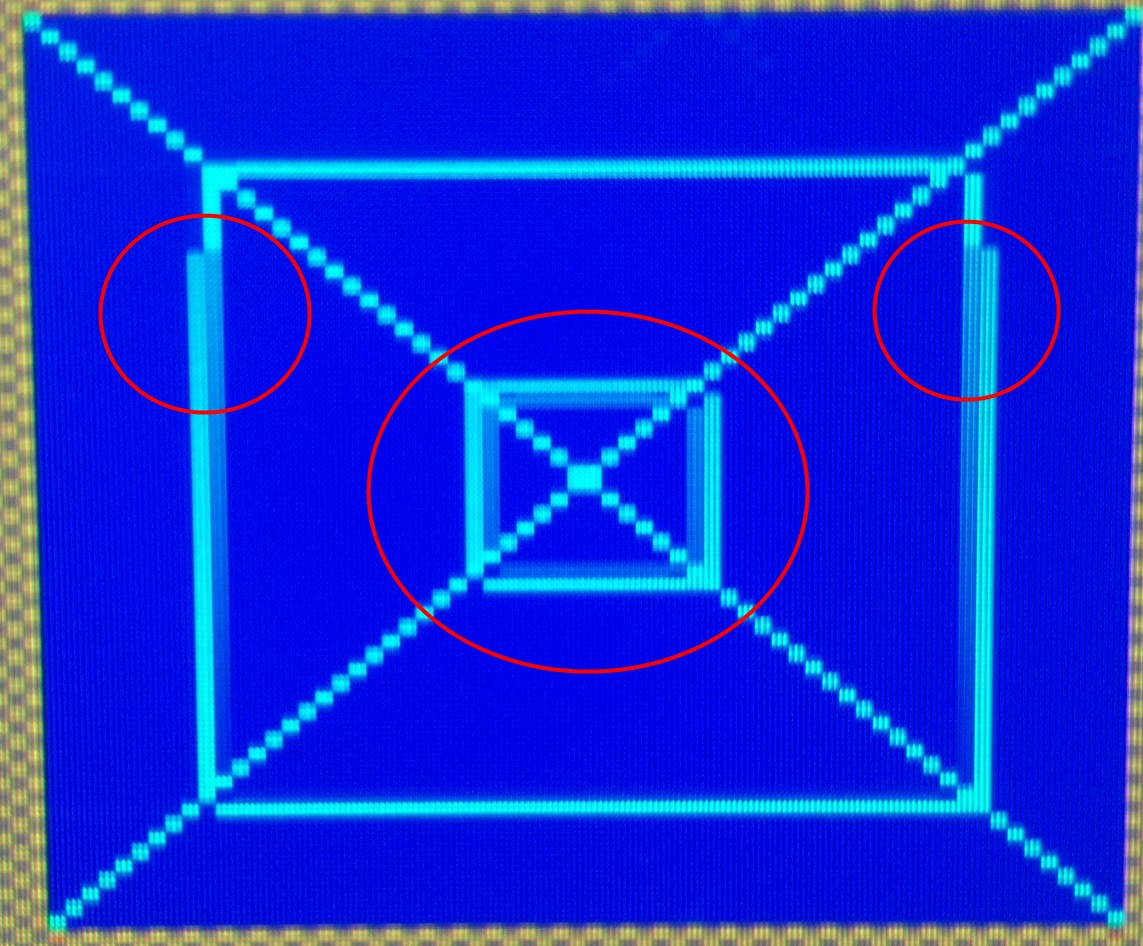
\includegraphics[width=0.5\textwidth]{../results/diagrams/single_buffering.png}
	\caption{Single buffering.}
	\label{fig:single_buffering}
\end{figure}
Double buffering is a technique to remove this artifact.
As the name implies two independent frame buffers are used.
While one frame buffer is being read and displayed on screen, 
the next frame is rendered to an off-screen frame buffer.
Once the frame has finished rendering the frame buffers are swapped, and the frame is displayed by the video unit.
In figure \ref{fig:double_buffering} it can be observed that double buffering improves the quality of the image substantially.
The image in the figure does have some artifacts, but the ones caused by single buffering are no longer present.
\begin{figure}[H]
	\centering
	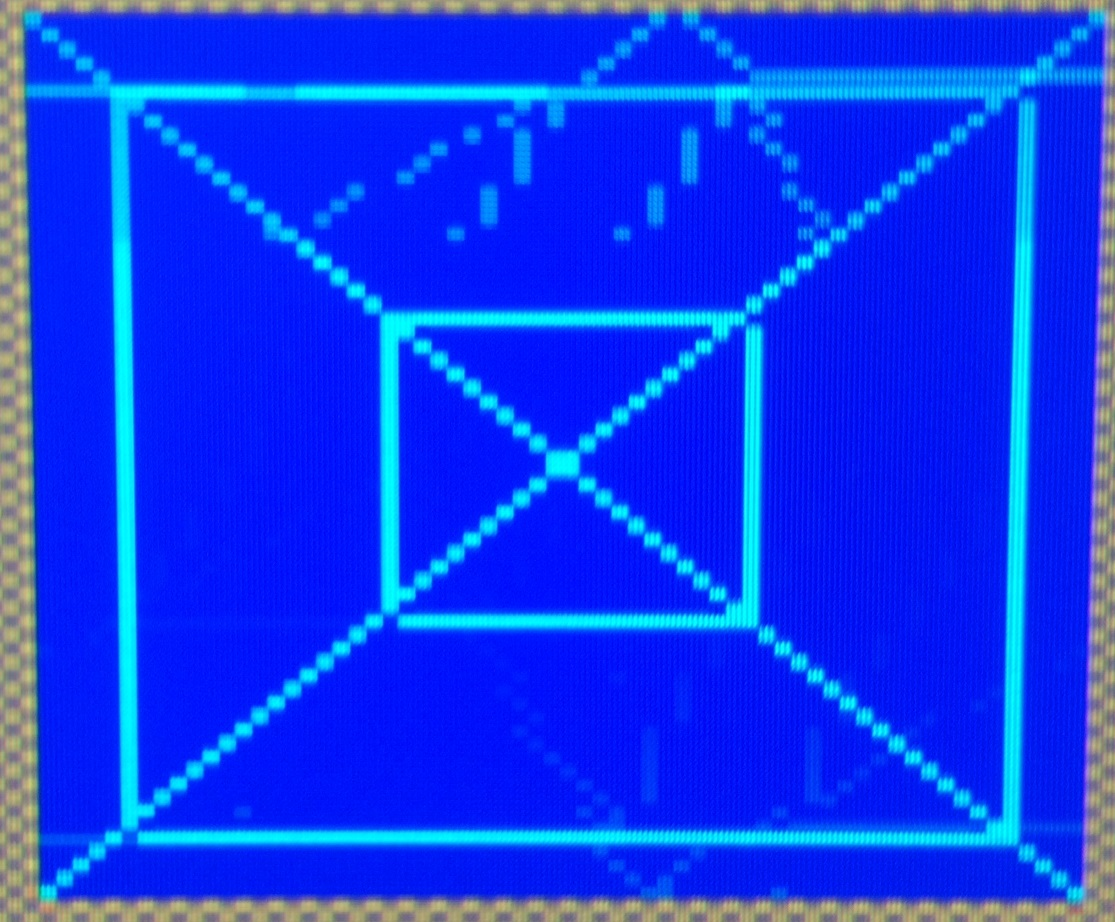
\includegraphics[width=0.5\textwidth]{../results/diagrams/double_buffering.png}
	\caption{Double buffering.}
	\label{fig:double_buffering}
\end{figure}

\section{Demolicious Power efficiency}

A Demolicious setup of 8 cores \ref{table:scalability} has a power draw of \SI{0.353}{W}.
By quickly and efficiently executing the kernel at hand, the GPU can reduce its total static power consumption.
Reducing the dynamic consumption however, is more difficult.
The current GPU architecture will execute nops when no kernels are active, keping dynamic power consumption sligthly lower than average, as no memory requests need to be served.
Therefore, Demolicious has been designed with the goal \ref{tab:goals} of allowing the host system to sleep as much as possible.

The Giant Gecko microcontroller used as the host device has four different energy modes, each lower energy mode more efficient, but more constrained.
Deeper power levels may conserve more power, but require a longer time to wake up.
EM0 is normal operation, while EM2 (Deep sleep mode) is the deepest power level with acceptable wake-up times for our usecase (somewhere around 2 ms) \cite{efm-referencemanual}.

There are two different sleep patterns used by the MCU based on the executing program:
\begin{enumerate}
  \item
    A visual animation or similar, rendering at a known target FPS.
    The MCU can stay at energy mode EM2 when kernels are executing, waking at fixed intervals to update and relaunch kernels.
  \item
    Programs working on some large dataset, where it is beneficial to tightly pack kernel execution, reducing GPU idling.
    The host device can therefore enter EM2 after launching a kernel, using the kernel complete pin to trigger an interrupt, waking the host device from sleep.
\end{enumerate}

The design is sound, and has been implemented successfully before by the authors,
but there was not enough time to fully implement it for this project in the host code.
ehe following numbers are therefore harvested from Silicon labs Simplicity studio energyAware Battery estimator.

Demolicous with 8 execution cores can run the tunnel kernel at 50 FPS @ 512x256, spending \SI{12.5}{ms} per frame \ref{fig:kernel_tunnel_fps}.
The tunnel kernel is to be executed 30 times per second, with the MCU waking via a timer interrupt to spawn the new kernels.
Kernel launch overhead is roughly $ 10\si\micro + 2 ms ~= 2 ms.$ When waking 30 times per second, this results in 60 ms awake per second.
EM0 with EBI consumes 142.6 mA, EM2 190\si\micro a. This then averages to roughly $ 142.6 mA * 0.060 + 0.19 mA * 0.940 = 8.734$ mA average consumption.

For the large dataset kernel, assume it takes 100ms to complete execution.
The MCU will have to wake 10 times per second, using 2 ms to wake and a negligible overhead to deploy new kernels.
This results in $ 10 * 2 ms = 20 ms $ spent in EM0, and 980 ms spent in EM2.
This averages to $ 142.6 mA * 0.020 + 0.19 mA * 0.980 = 3.038 mA $ average consumption.

Without any use of sleep mode for the MCU, the 142.6 mA drawn make for a total power consumption of $142.6 mA * 3.3V = 470.6 mW $.
However, for the tunnel kernel example, making use of sleep mode puts the power consumption at $ 8.734 mA * 3.3V = 28.8mW$. 
For the large dataset kernel, power consumption is at $ 3.038 mA * 3.3V = 10.0 mW$.

These results show that there is a clear gain to be had from introducing low power modes. 

\subsection*{Power budget}

The computer is powered by a EH-70p USB charger for the Nikon Coolpix S2700 camera \cite[p. 196]{usb-charger}.
This charger outputs a 5 V voltage and delivers 550 mA.
This gives the power input an upper bound of power consumption at $550mA * 5V = 2.75W$.

Based on checking the memory datasheet \cite{SRAM-datasheet}, page 4, the average current drawn from the SRAM is 100mA.
At two components, the memory energy consumption becomes $2 * 100mA * 3.3V = 660mW$, which makes them the most energy demanding part of the computer. 

With these major components and their estimated power consumption, one can see that the final system draws approximately $ 660mW + 353mW + 28mW = 1041mW $. The total power consumed is likely a little higher on account of signal propagation, but it is still significantly less than the $2.75 W$ we accounted for in the power design.

\end{document}
